        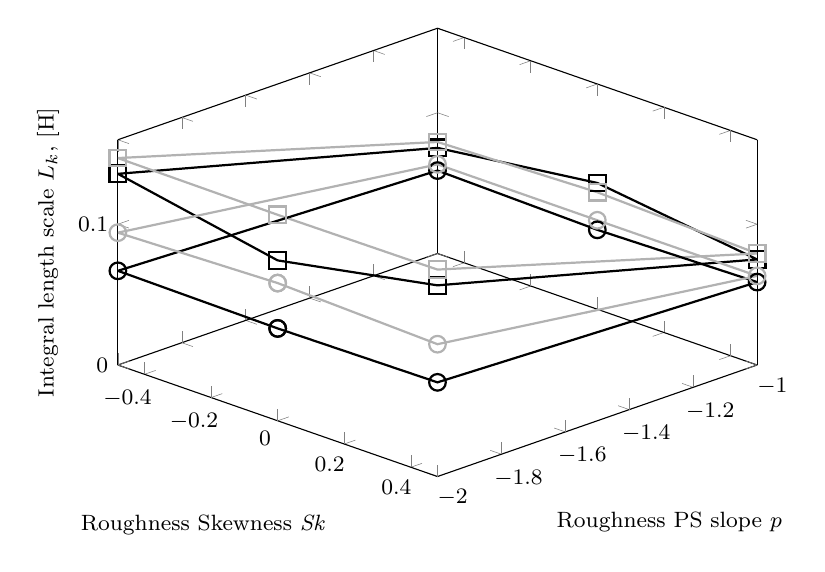
\begin{tikzpicture}[]
        \centering
        \begin{axis}[
        view={45}{35},
            ylabel={Roughness PS slope $p$},
            xlabel={Roughness Skewness \textit{Sk}},
			zlabel={Integral length scale $L_k$, [H]},
			%ztick={5.5,6,6.5,7,7.5},
			zmin=0,zmax=0.16,
            %ymin=0, ymax=0.16,
            width=.8\textwidth,
            height=.6\textwidth,
            label style={font=\footnotesize},
            tick label style={font=\footnotesize}
            ]
                        \addplot3 [
            black,mark=square,thick, mark size=3pt
            ]
            coordinates{
            (0,-2,0.1139)			
			(0.48,-2,0.1358)
			(0.48,-1,0.075)
			(0,-1,0.0897)
			(-0.48,-1,0.075)
			(-0.48,-2,0.1358)
            (0,-2,0.1139)
			};
			\addplot3 [
            gray!60,mark=square,thick, mark size=3pt
            ]
            coordinates{
            
            (0,-2,0.1463)
			(0.48,-2,0.147)
			(0.48,-1,0.0792)
			(0,-1,0.0831)
			(-0.48,-1,0.0792)
			(-0.48,-2,0.147)
			(0,-2,0.1463)
            };
            
                                    \addplot3 [
            black,mark=o,thick, mark size=3pt
            ]
            coordinates{
            (0,-2,0.0656)			
			(0.48,-2,0.0669)
			(0.48,-1,0.0589)
			(0,-1,0.0564)
			(-0.48,-1,0.0589)
			(-0.48,-2,0.0669)
            (0,-2,0.0656)
			};
			
			
			\addplot3 [
            gray!60,mark=o,thick, mark size=3pt
            ]
            coordinates{
            
            (0,-2,0.0978)
			(0.48,-2,0.094)
			(0.48,-1,0.0633)
			(0,-1,0.0632)
			(-0.48,-1,0.0633)
			(-0.48,-2,0.094)
			(0,-2,0.0978)
            };
            
            
            
            
            
        \end{axis}
        \end{tikzpicture}